\documentclass[serif,mathserif]{beamer}
\usepackage[portuguese]{babel}
\usepackage[utf8]{inputenc}
\usepackage{amsmath, amsfonts, epsfig, xspace}
\usepackage{algorithm,algorithmic}
\usepackage{pstricks,pst-node}
\usepackage{multimedia}
\usepackage[normal,tight,center]{subfigure}
\setlength{\subfigcapskip}{-.5em}
\usepackage[font=scriptsize]{caption} %Diminuindo tamanho da caption
\usepackage{beamerthemesplit}
\usetheme{lankton-keynote}
\setbeamerfont{title}{size=\large}

\newcommand{\CcImageBy}[1]{%
  
\includegraphics[scale=#1]{src/img/creative_commons/cc_by_30.pdf}%
}
\newcommand{\CcImageSa}[1]{%
  
\includegraphics[scale=#1]{src/img/creative_commons/cc_sa_30.pdf}%
}
\newcommand{\CcGroupBySa}[2]{% zoom, gap
  \CcImageBy{#1}\hspace*{#2}\CcImageSa{#1}%
}
\newcommand{\CcLongnameBySa}{Attribution-ShareAlike}
\newcommand{\CcNote}[1]{% longname
  This work is licensed under the \textit{Creative Commons #1 3.0 License}.%
}

\author[Alessandro Palmeira\\ \and Itai Soares]{Alessandro Palmeira\\ \and Itai Soares}

\title[Instituto de Matemática e Estatística - USP\hspace{2em}\insertframenumber/\inserttotalframenumber]{Acompanhamento musical em tempo real utilizando múltiplas performances como referência}

\date{22 de Setembro de 2016} %leave out for today's date to be insterted

\institute{MAC6917 Topics in Sound and Music Computing: Music Information Retrieval}


\begin{document}


\begin{frame}
  \titlepage
  \begin{center}
    \CcGroupBySa{0.83}{0.95ex}\\
    {\tiny\CcNote{\CcLongnameBySa}}
  \end{center}
\end{frame}

\section{Apresentação}
\begin{frame}
  \frametitle{Apresentação}
  Este seminário será uma apresentação do artigo \emph{Real-time music tracking using multiple performances as a reference} de Andreas Arzt e Gerhard Widmer que ganhou o \emph{Best Paper Award} na  \emph{International Society for Music Information Retrieval Conference} de 2015.
\end{frame}

\section{Introdução}  % add these to see outline in slides

\begin{frame}
  \frametitle{Algoritmos de Acompanhamento em Tempo Real}
  Existem desde a década de 1980 e ainda atraem bastante pesquisa.\pause\\
  Essa tecnologia tem sido usado em aplicações práticas.\pause
  %Colocar vídeo do SmartMusic(1985) aqui
  \begin{itemize}
    \item Antescofo\\
    \item Tonara
  \end{itemize}
\end{frame}

\begin{frame}
  \frametitle{Estratégias utilizadas}
  \begin{itemize}
    \item Inicia-se com uma representação simbólica, como um arquivo MIDI ou MusicXML\\\pause
    \item Converte-o para um arquivo de áudio, usando um softare sintetizador\pause
      \begin{itemize}
        \item O problema se reduz a um alinhamento áudio-áudio\\\pause
        \item Sabe-se o tempo de cada evento\\
      \end{itemize}
  \end{itemize}
\end{frame}

\begin{frame}
  \frametitle{Nova estratégia}
  \begin{itemize}
    \item Primeiramente utilizamos uma outra performance da música e a alinhamos com a partitura de forma automatizada\\\pause
    \item Depois, utilizamos essa ``performance anotada'' como nova representação para o processo de rastreamento online\pause
  \end{itemize}

  %inserir figura src/img/2-Figure1-1.png

%\vspace{5mm} %5mm vertical space

  As motivações são:\pause
  \begin{itemize}
    \item Qualidade das características extraídas\\\pause % O arquivo de áudio tem qualidade maior do que uma síntese
    \item Complexidade perdida na notação musical, que aparece em uma performance\pause % Como trilos, por exemplo
  \end{itemize}
  Porém, temos também uma desvantagem:\pause
  \begin{itemize}
    \item A qualidade do processo fica dependente da performance\\
  \end{itemize}
\end{frame}

\begin{frame}[label=figura1]
  \frametitle{Nova estratégia}
  \begin{figure}[!ht]
    \centering
    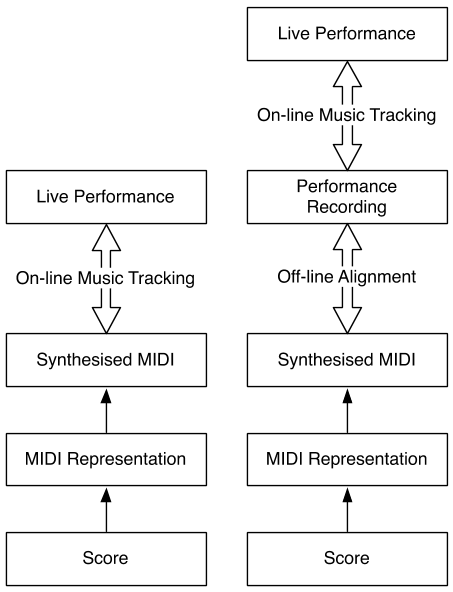
\includegraphics[height=0.7\textheight]{src/img/2-Figure1-1.png}
    \caption*{Rastreamento padrão (esquerda), rastreamento utilizando uma performance como referência (direita)}
  \end{figure}
\end{frame}


\section{Desenvolvimento}
\begin{frame}
  \frametitle{Descrição dos dados}
  \pause
  \begin{center}
    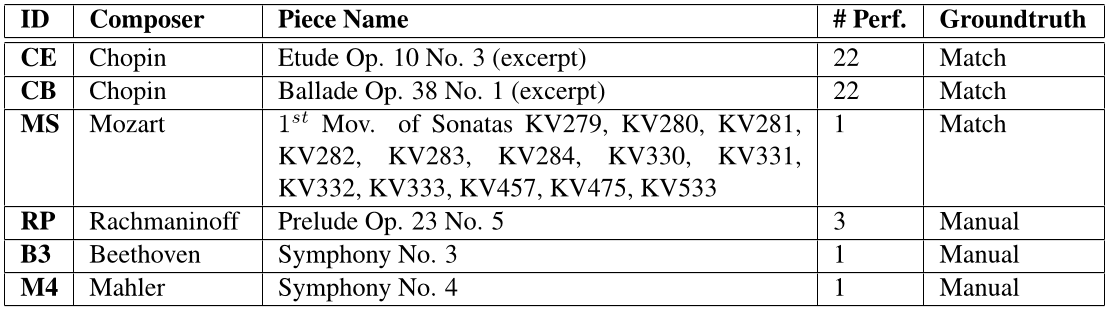
\includegraphics[width=\textwidth]{src/img/1-Table1-1.png}
  \end{center}
% As músicas automáticas foram gravadas com um piano MIDI
% As músicas anotadas foram anotadas manulmente, no nível de nota no rachmaninoff
% e pulso para as sinfonias
% 7 Performances adicionais foram coletadas sem anotação, apenas para serem processadas de forma automática. Com exceção das que já tem 22 (7 foram escolhidas aleatoriamente dentre elas, sem repetir o performer)
%(dizer que existem duas musicas orquestrais, dificuldade maior)
%    (dizer que foi obtido mais de uma gravação da mesma musica)
\end{frame}

\begin{frame}
  \frametitle{Rastreamento padrão baseado em representação simbólica musical}
  Abordagem baseada no algoritmo \emph{Dynamic Time Warping (DTW)} com algumas extensões:\pause % que possibilitam a aplicação em rastreamento online. [artigo 10]
  \begin{itemize}
    \item O caminho é computado de maneira incremental\\\pause
    \item A complexidade é reduzida para ser linear no tamanho da entrada\pause
    \item Utiliza a estratégia \emph{backward-forward} %reconsidera decisoes passadas, aumenta robustez [artigo 4] % aumenta a habilidade de o algoritmo lidar com diferencas no Andamento [artigo 3]
  \end{itemize}
\end{frame}

\begin{frame}
  \frametitle{Rastreamento padrão baseado em representação simbólica musical}
  % Para ser possível o tracking é necessário...
  Precisamos de uma representação da partitura\pause
  \begin{itemize}
    \item Síntese MIDI -> áudio\\\pause
    \item Alinhamento áudio-áudio, agora com a informação temporal de cada nota\pause
  \end{itemize}
  Nesse artigo, é usado uma mistura de características cromáticas e de início de nota \emph{(semi-tone onset)} e o algoritmo explicado anteriormente
\end{frame}

\begin{frame}
  \frametitle{Resultados utilizando o rastreamento padrão}
  \begin{center}
    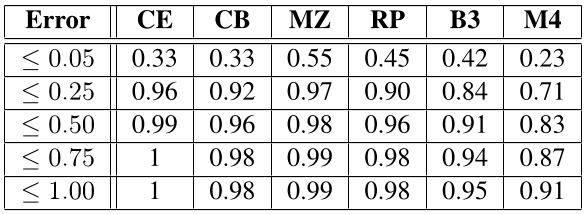
\includegraphics[width=0.8\textwidth]{src/img/1-Table2-1.png}
  \end{center}
  \pause
  \begin{itemize}
    \item Funciona bem para peças em piano\\\pause
    \item Não funciona bem para peças orquestrais
    %É fácil sintetizar piano mas é muito mais complexo para orquestras
  \end{itemize}
\end{frame}

\begin{frame}
  \frametitle{Rastreamento utilizando uma performance como referência}
  O rastreamento padrão funciona bem mas ganhamos algumas vantagens ao utilizar uma performance real como referência:\pause
  \begin{itemize}
    \item Melhor qualidade\pause
    \item Características mais próximas da performance ao vivo que queremos rastrear\pause
    \item Maior similaridade sonora, principalmente em peças orquestradas\pause
    \item Informações detalhadas de andamento, dinâmica e articulação
  \end{itemize}
\end{frame}

\begin{frame}
  \frametitle{Rastreamento utilizando uma performance como referência}
  Porém, temos uma grande desvantagem:\pause
  \begin{itemize}
    \item A informação temporal das notas é inexistente\pause
  \end{itemize}
  Assim, precisaremos calcular esta informação para seguir essa abordagem. \pause Nesse artigo, isso será feito de forma automática
\end{frame}

\againframe<1>{figura1}

\begin{frame}
  \frametitle{Alinhamento off-line}
  \begin{itemize}
    \item Espera-se que o aumento na qualidade das características supere o erro introduzido por esta etapa\pause
    \item Aqui, usamos o algoritmo já citado, com a única diferença de que, no final, computamos o caminho contrário, como se faz no DTW padrão.
    % É claro que podemos usar qualquer algoritmo de alinhamento
  \end{itemize}
  Assim, temos resultados melhores que o caso online.
\end{frame}

\begin{frame}
  \frametitle{Comparação dos resultados}

  \begin{figure}[!tbp]
    \centering
    \begin{minipage}[b]{0.45\textwidth}
      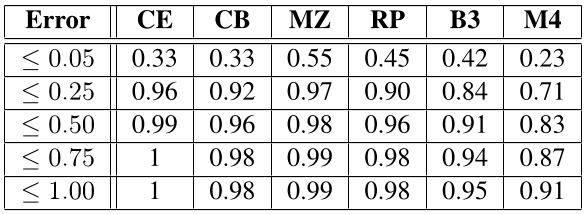
\includegraphics[width=\textwidth]{src/img/1-Table2-1.png}
      \caption*{Rastreamento padrão}
    \end{minipage}
    \hfill
    \begin{minipage}[b]{0.45\textwidth}
      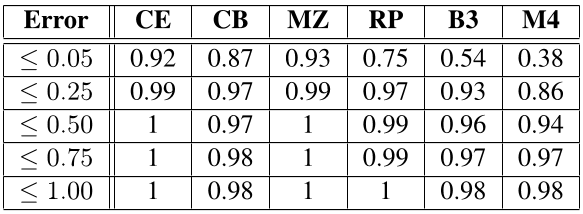
\includegraphics[width=\textwidth]{src/img/1-Table3-1.png}
      \caption*{Alinhamento off-line}
    \end{minipage}
  \end{figure}
\end{frame}

\begin{frame}
  \frametitle{Rastreamento baseado em uma performance alinhada}
  Agora, utilizando a performance já alinhada, utilizamos o mesmo algoritmo de rastreamento para as outras performances.
  Estes são os resultados:
  \begin{figure}[!ht]
    \centering
    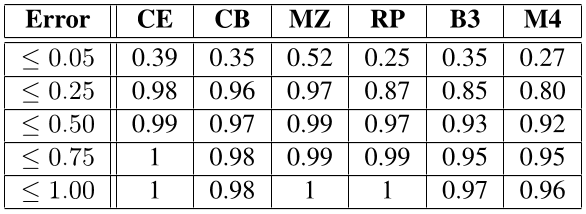
\includegraphics[width=0.7\textwidth]{src/img/3-Table4-1.png}
    \caption*{Rastreamento on-line baseado em uma performance alinhada off-line}
  \end{figure}
\end{frame}

\begin{frame}
  \frametitle{Rastreamento baseado em uma performance alinhada}
  \begin{itemize}
    \item Melhoria nas peças orquestradas\pause
    \item Resultados se mostraram instáveis - algumas performances são mais similares entre si do que com a usada como referência \pause %Infelizmente
    \item Resultados mostraram que algumas partes da peça tiveram erros frequentemente \pause %A peça é difícil mesmo
    \item Utilizando diferentes performances como referência, alguns erros só apareciam em uma ou duas delas \pause
  \end{itemize}
  Isto levou à ideia de combinar o alinhamento de várias performances para diminuir estes erros.
\end{frame}

\begin{frame}[label=figura2]
  \frametitle{Rastreamento baseado em várias performances alinhadas}
  \begin{figure}[!ht]
    \centering
    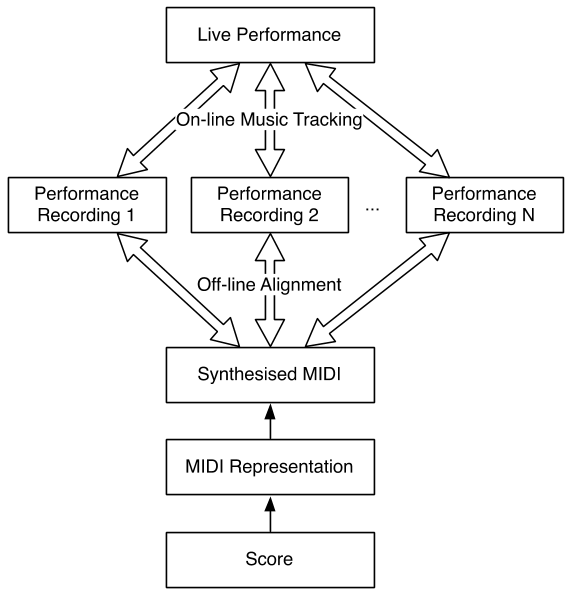
\includegraphics[height=0.7\textheight]{src/img/2-Figure2-1.png}
    \caption*{Rastreamento multi-agente baseado em várias performances alinhadas off-line}
  \end{figure}
\end{frame}

\begin{frame}
  \frametitle{Rastreamento baseado em múltiplas performances}
  \begin{itemize}
    \item Várias anotações alinhadas são usadas em paralelo no rastreamento\pause
    \item Utilizamos a mediana \pause %Explicar o porquê
    \item Mais estabilidade em aplicações práticas \pause
    \item Foram utilizadas 7 performances\pause %explicar tradeoff robustez x tempo de computação
  \end{itemize}
\end{frame}

\section{Resultados}
\begin{frame}
  \frametitle{Comparação dos resultados}

  \begin{figure}[!tbp]
    \centering
    \begin{minipage}[b]{0.45\textwidth}
      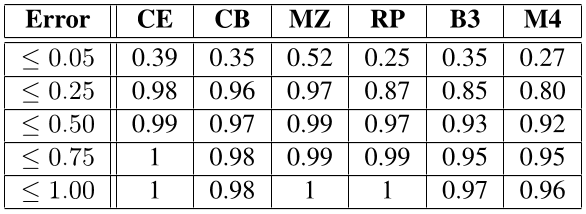
\includegraphics[width=\textwidth]{src/img/3-Table4-1.png}
      \caption*{Apenas uma performance como referência}
    \end{minipage}
    \hfill
    \begin{minipage}[b]{0.45\textwidth}
      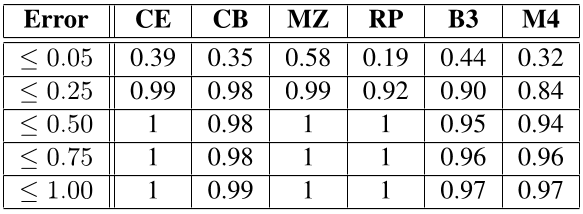
\includegraphics[width=\textwidth]{src/img/3-Table5-1.png}
      \caption*{Múltiplas performances como referência}
    \end{minipage}
  \end{figure}
\end{frame}

\begin{frame}
  \frametitle{Comparação de todos os resultados}
  \begin{center}
    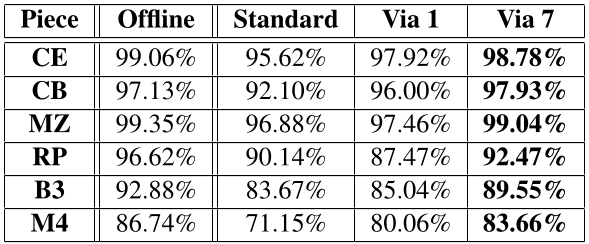
\includegraphics[width=0.8\textwidth]{src/img/4-Table6-1.png}
  \end{center}
  \begin{itemize}
    \item Melhores resultados do que o alinhamento off-line\pause
    \item Erros introduzidos no alinhamento off-line impactaram menos do que a melhora de qualidade no método
  \end{itemize}
\end{frame}

\section{Cenário real}
\begin{frame}
  \frametitle{Projeto PHENICX}
  \begin{itemize}
    \item Projeto que visa melhorar a experiência da música clássica\pause
    \item Videodock criou a interface de usuário e as visualizações \pause
  \end{itemize}
  O grande evento: \pause
  \begin{itemize}
    \item Dia 7 de Fevereiro de 2015\pause
    \item Concertgebouw - Amsterdam\pause
    \item The Royal Concertgebouw Orchestra, conduzida por Semyon Bychkov\pause
    \item Alpensinfonie - Richard Strauss\pause
    \item Nenhum acesso à representação simbólica - Anotação feita à mão (downbeat) para uma performance\pause
    \item Outras 6 performances alinhadas com essa primeira
  \end{itemize}
\end{frame}


\section{Conclusão}
\begin{frame}
  \frametitle{Melhorias futuras}
  \begin{itemize}
    \item Melhorar o rastreamento com apenas uma performance\pause
    \item Melhorar rastreamento em partes com diferença entre partitura e gravação \pause
    \item Usar mais do que 7 performances como referência \pause
    \item Focar no problema de escolher as melhores performances gravadas para uma certa performance ao vivo \pause
    \item Buscar alternativas para a escolha da mediana
  \end{itemize}
\end{frame}

\begin{frame}
  \frametitle{Dúvidas?}
  \begin{itemize}
    \item Os slides estão disponíveis em \url{https://github.com/compmusMIR}
  \end{itemize}
\end{frame}

\begin{frame}
  \frametitle{Referências}
  \small
  Apresentação:\\
  \vspace{2mm}
  \url{https://www.semanticscholar.org/paper/Real-Time-Music-Tracking-Using-Multiple-Arzt-Widmer/0223b9d27de14f2c158028290782a937ff537786}


\end{frame}

\end{document}
